\documentclass[a4paper,11pt,titlepage]{article}

\usepackage[utf8]{inputenc}
\usepackage[T1]{fontenc}
\usepackage[english]{babel}
\usepackage{color}
\usepackage{xcolor}
\usepackage{graphicx}
\usepackage{amsmath}
\usepackage{amssymb}
\usepackage{mathtools}
\usepackage{stmaryrd}
\usepackage[hmargin={2.5cm,2.5cm},top=2.5cm,bottom=2.5cm]{geometry}
\usepackage{lmodern}
\usepackage[ruled,lined]{algorithm2e}
\usepackage{listings}
\usepackage{tikz, pgf}

\usepackage{tikz-uml}

\usepackage[colorlinks=true,breaklinks=true,linkcolor=blue,filecolor=magenta,urlcolor=cyan,pdftitle={Project},pdfsubject={Project}]{hyperref}

\usetikzlibrary{arrows,shapes,positioning}

\sloppy
\hyphenpenalty 10000000

\title{AP4B Project Template}
\author{blah}

\begin{document}

    \maketitle
    \newpage

    \tableofcontents
    \newpage

    \section{Introduction}\label{sec:introduction}

    \begin{align*}
        x = 2 &\implies x²=4 \text{ dtdtdtdt}
    \end{align*}

    \verb|azerxdrsdr5|


    \begin{center}
        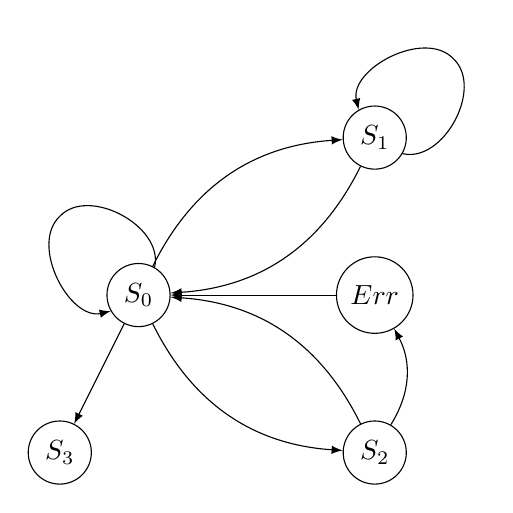
\begin{tikzpicture}
            \node[draw, circle] (S0) at (-1,0) {$S_0$} ;
            \node[draw, circle] (S1) at (2,2) {$S_1$} ;
            \node[draw, circle] (S2) at (2,-2) {$S_2$} ;
            \node[draw, circle] (S3) at (-2,-2) {$S_3$} ;
            \node[draw, circle] (Err) at (2,0) {$Err$} ;

            \draw (S0) to[bend right=75](-2,1);
            \draw[->,>=latex](-2,1) to[bend right=75](S0);

            \draw[->,>=latex] (S0) edge[bend left] (S1) ;
            \draw[->,>=latex] (S0) edge[bend right] (S2) ;
            \draw[->,>=latex] (S0) edge (S3) ;

            \draw[->,>=latex] (S1) edge[bend left] (S0) ;
            \draw (S1) to[bend right=75](3,3);
            \draw[->,>=latex](3,3) to[bend right=75](S1);

            \draw[->,>=latex] (S2) edge[bend right] (S0) ;
            \draw[->,>=latex] (S2) edge[bend right] (Err) ;

            \draw[->,>=latex] (Err) edge (S0) ;
        \end{tikzpicture}
    \end{center}

    \begin{center}
        \begin{tikzpicture}
            \begin{umlpackage}{p}
                \begin{umlpackage}{sp1}
                    \umlclass[template=T]{A}{
                        n : uint \\ t : float
                    }{n}
                    \umlclass[y=-3]{B}{
                        d : double
                    }{
                        \umlvirt{setB(b : B) : void} \\ getB() : B}
                \end{umlpackage}
                \begin{umlpackage}[x=10,y=-6]{sp2}
                    \umlinterface{C}{
                        n : uint \\ s : string
                    }{}
                \end{umlpackage}
                \umlclass[x=2,y=-10]{D}{
                    n : uint
                }{}
            \end{umlpackage}

            \umlassoc[geometry=-|-, arg1=tata, mult1=*, pos1=0.3, arg2=toto, mult2=1, pos2=2.9, align2=left]{C}{B}
            \umlunicompo[geometry=-|, arg=titi, mult=*, pos=1.7, stereo=vector]{D}{C}
            \umlimport[geometry=|-, anchors=90 and 50, name=import]{sp2}{sp1}
            \umlaggreg[arg=tutu, mult=1, pos=0.8, angle1=30, angle2=60, loopsize=2cm]{D}{D}
            \umlinherit[geometry=-|]{D}{B}
            \umlnote[x=2.5,y=-6, width=3cm]{B}{Je suis une note qui concerne la classe B}
            \umlnote[x=7.5,y=-2]{import-2}{Je suis une note qui concerne la relation d'import}
        \end{tikzpicture}
    \end{center}

\end{document}